\documentclass{standalone}
\usepackage{tikz}
\usetikzlibrary{patterns, positioning}


\begin{document}
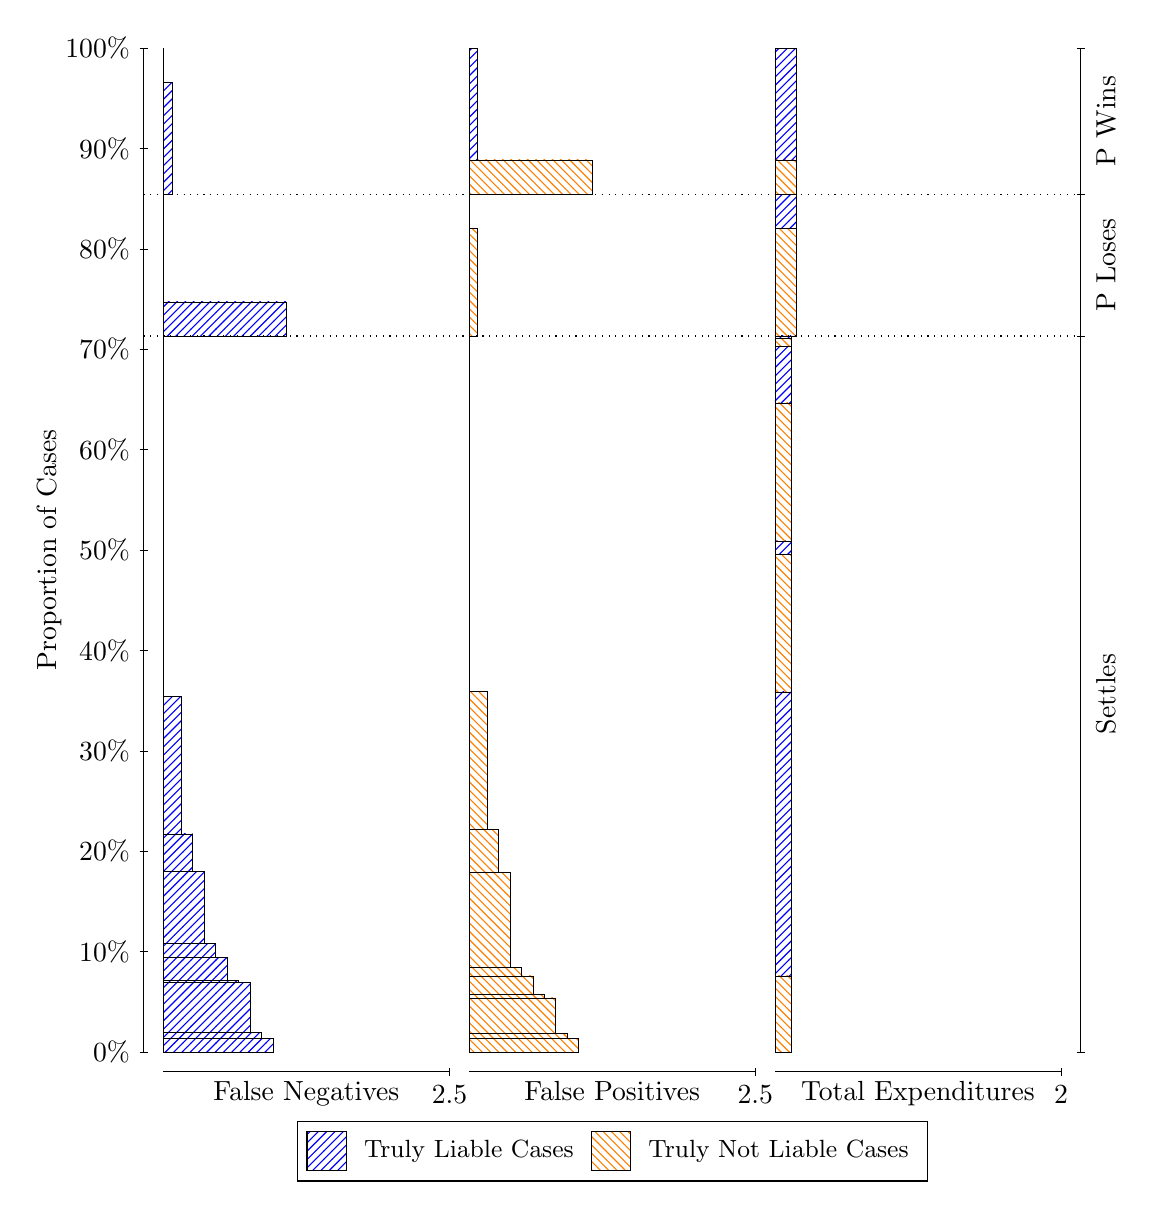
\begin{tikzpicture}
\draw[black, very thin] (1.5,1.75) -- (1.5,14.5);
\node[rotate=90, text=black, anchor=center] at (0.3, 8.125) {Proportion of Cases};
\draw[black, very thin] (1.45,1.75) -- (1.55,1.75);
\node[text=black, anchor=east] at (1.45, 1.75) {0\%};
\draw[black, very thin] (1.45,3.025) -- (1.55,3.025);
\node[text=black, anchor=east] at (1.45, 3.025) {10\%};
\draw[black, very thin] (1.45,4.3) -- (1.55,4.3);
\node[text=black, anchor=east] at (1.45, 4.3) {20\%};
\draw[black, very thin] (1.45,5.575) -- (1.55,5.575);
\node[text=black, anchor=east] at (1.45, 5.575) {30\%};
\draw[black, very thin] (1.45,6.85) -- (1.55,6.85);
\node[text=black, anchor=east] at (1.45, 6.85) {40\%};
\draw[black, very thin] (1.45,8.125) -- (1.55,8.125);
\node[text=black, anchor=east] at (1.45, 8.125) {50\%};
\draw[black, very thin] (1.45,9.4) -- (1.55,9.4);
\node[text=black, anchor=east] at (1.45, 9.4) {60\%};
\draw[black, very thin] (1.45,10.675) -- (1.55,10.675);
\node[text=black, anchor=east] at (1.45, 10.675) {70\%};
\draw[black, very thin] (1.45,11.95) -- (1.55,11.95);
\node[text=black, anchor=east] at (1.45, 11.95) {80\%};
\draw[black, very thin] (1.45,13.225) -- (1.55,13.225);
\node[text=black, anchor=east] at (1.45, 13.225) {90\%};
\draw[black, very thin] (1.45,14.5) -- (1.55,14.5);
\node[text=black, anchor=east] at (1.45, 14.5) {100\%};

\draw[black, very thin] (13.4,1.75) -- (13.4,14.5);
\draw[black, very thin] (13.35,1.75) -- (13.45,1.75);
\node[anchor=west] at (13.35, 1.75) {};
\draw[black, very thin] (13.35,10.843) -- (13.45,10.843);
\node[anchor=west] at (13.35, 10.843) {};
\draw[black, very thin] (13.35,12.644) -- (13.45,12.644);
\node[anchor=west] at (13.35, 12.644) {};
\draw[black, very thin] (13.35,14.5) -- (13.45,14.5);
\node[anchor=west] at (13.35, 14.5) {};

\draw[black, very thin, pattern color=blue, pattern=north east lines] (1.75,1.75) rectangle (3.1398,1.9182);
\draw[black, very thin, pattern color=blue, pattern=north east lines] (1.75,1.9182) rectangle (2.9944,1.9979);
\draw[black, very thin, pattern color=blue, pattern=north east lines] (1.75,1.9979) rectangle (2.8491,2.6308);
\draw[black, very thin, pattern color=blue, pattern=north east lines] (1.75,2.6308) rectangle (2.7037,2.6609);
\draw[black, very thin, pattern color=blue, pattern=north east lines] (1.75,2.6609) rectangle (2.5584,2.9496);
\draw[black, very thin, pattern color=blue, pattern=north east lines] (1.75,2.9496) rectangle (2.4131,3.1295);
\draw[black, very thin, pattern color=blue, pattern=north east lines] (1.75,3.1295) rectangle (2.2678,4.0472);
\draw[black, very thin, pattern color=blue, pattern=north east lines] (1.75,4.0472) rectangle (2.1224,4.5203);
\draw[black, very thin, pattern color=blue, pattern=north east lines] (1.75,4.5203) rectangle (1.9771,6.2688);
\draw[black, very thin, pattern color=orange, pattern=north west lines] (1.75,6.2688) rectangle (1.75,10.843);
\draw[black, very thin, pattern color=blue, pattern=north east lines] (1.75,10.843) rectangle (3.3123,11.277);
\draw[black, very thin, pattern color=orange, pattern=north west lines] (1.75,11.277) rectangle (1.75,12.644);
\draw[black, very thin, pattern color=blue, pattern=north east lines] (1.75,12.644) rectangle (1.859,14.066);
\draw[black, very thin, pattern color=orange, pattern=north west lines] (1.75,14.066) rectangle (1.75,14.5);
\draw[black, very thin, pattern color=orange, pattern=north west lines] (5.6333,1.75) rectangle (7.0231,1.9182);
\draw[black, very thin, pattern color=orange, pattern=north west lines] (5.6333,1.9182) rectangle (6.8777,1.9824);
\draw[black, very thin, pattern color=orange, pattern=north west lines] (5.6333,1.9824) rectangle (6.7324,2.4367);
\draw[black, very thin, pattern color=orange, pattern=north west lines] (5.6333,2.4367) rectangle (6.5871,2.4823);
\draw[black, very thin, pattern color=orange, pattern=north west lines] (5.6333,2.4823) rectangle (6.4417,2.7153);
\draw[black, very thin, pattern color=orange, pattern=north west lines] (5.6333,2.7153) rectangle (6.2964,2.8213);
\draw[black, very thin, pattern color=orange, pattern=north west lines] (5.6333,2.8213) rectangle (6.1511,4.029);
\draw[black, very thin, pattern color=orange, pattern=north west lines] (5.6333,4.029) rectangle (6.0057,4.576);
\draw[black, very thin, pattern color=orange, pattern=north west lines] (5.6333,4.576) rectangle (5.8604,6.3246);
\draw[black, very thin, pattern color=blue, pattern=north east lines] (5.6333,6.3246) rectangle (5.6333,10.843);
\draw[black, very thin, pattern color=orange, pattern=north west lines] (5.6333,10.843) rectangle (5.7423,12.21);
\draw[black, very thin, pattern color=blue, pattern=north east lines] (5.6333,12.21) rectangle (5.6333,12.644);
\draw[black, very thin, pattern color=orange, pattern=north west lines] (5.6333,12.644) rectangle (7.1957,13.078);
\draw[black, very thin, pattern color=blue, pattern=north east lines] (5.6333,13.078) rectangle (5.7423,14.5);
\draw[black, very thin, pattern color=orange, pattern=north west lines] (9.5167,1.75) rectangle (9.721,2.7153);
\draw[black, very thin, pattern color=blue, pattern=north east lines] (9.5167,2.7153) rectangle (9.721,6.3232);
\draw[black, very thin, pattern color=orange, pattern=north west lines] (9.5167,6.3232) rectangle (9.721,8.0718);
\draw[black, very thin, pattern color=blue, pattern=north east lines] (9.5167,8.0718) rectangle (9.721,8.24);
\draw[black, very thin, pattern color=orange, pattern=north west lines] (9.5167,8.24) rectangle (9.721,9.9947);
\draw[black, very thin, pattern color=blue, pattern=north east lines] (9.5167,9.9947) rectangle (9.721,10.707);
\draw[black, very thin, pattern color=orange, pattern=north west lines] (9.5167,10.707) rectangle (9.721,10.813);
\draw[black, very thin, pattern color=blue, pattern=north east lines] (9.5167,10.813) rectangle (9.721,10.843);
\draw[black, very thin, pattern color=orange, pattern=north west lines] (9.5167,10.843) rectangle (9.7892,12.21);
\draw[black, very thin, pattern color=blue, pattern=north east lines] (9.5167,12.21) rectangle (9.7892,12.644);
\draw[black, very thin, pattern color=orange, pattern=north west lines] (9.5167,12.644) rectangle (9.7892,13.078);
\draw[black, very thin, pattern color=blue, pattern=north east lines] (9.5167,13.078) rectangle (9.7892,14.5);
\draw[black, dotted] (1.5,10.843) -- (13.4,10.843);
\draw[black, dotted] (1.5,12.644) -- (13.4,12.644);
\draw[black, very thin] (1.75,1.5) -- (5.3833,1.5);
\node[text=black, anchor=north] at (3.5667, 1.5) {False Negatives};
\draw[black, very thin] (5.3833,1.45) -- (5.3833,1.55);
\node[text=black, anchor=north] at (5.3833, 1.45) {2.5};

\draw[black, very thin] (5.6333,1.5) -- (9.2667,1.5);
\node[text=black, anchor=north] at (7.45, 1.5) {False Positives};
\draw[black, very thin] (9.2667,1.45) -- (9.2667,1.55);
\node[text=black, anchor=north] at (9.2667, 1.45) {2.5};

\draw[black, very thin] (9.5167,1.5) -- (13.15,1.5);
\node[text=black, anchor=north] at (11.333, 1.5) {Total Expenditures};
\draw[black, very thin] (13.15,1.45) -- (13.15,1.55);
\node[text=black, anchor=north] at (13.15, 1.45) {2};

\node[text=black, centered, rotate=90] at (13.72, 6.2967) {Settles};
\node[text=black, centered, rotate=90] at (13.72, 11.744) {P Loses};
\node[text=black, centered, rotate=90] at (13.72, 13.572) {P Wins};

\draw (7.449999999999999,1.5) node[draw=none] (baseCoordinate) {};
\begin{scope}[align=center]
        \matrix[scale=0.5, draw=black, below=0.5cm of baseCoordinate, nodes={draw}, column sep=0.1cm]{
            \node[rectangle, draw, minimum width=0.5cm, minimum height=0.5cm, pattern color=blue, pattern=north east lines] {}; &
            \node[draw=none, font=\small, text=black] (B) {Truly Liable Cases}; &
            \node[rectangle, draw, minimum width=0.5cm, minimum height=0.5cm, pattern color=orange, pattern=north west lines] {}; &
            \node[draw=none, font=\small, text=black] (B) {Truly Not Liable Cases}; \\
            };
\end{scope}

\end{tikzpicture}
\end{document}